\documentclass[]{subfiles}

\begin{document}

我们有:
\begin{align*}
z = & w^T X + b \\
a = & \sigma(z)
\end{align*}

计算梯度:
\begin{align*}
\frac{\partial \mathcal{L}}{\partial w}
= & \frac{\partial z}{\partial w}
    \frac{\partial a}{\partial z}
    \frac{\partial \mathcal{L}}{\partial a} \\
= & X^T \cdot \sigma'(z) \cdot
    \frac{\partial \mathcal{L}}{\partial a}
\end{align*}
考虑到:
\begin{align*}
x_i > 0, \forall x_i \in X \\
\sigma'(z) > 0
\end{align*}
故:
$$
sign(\frac{\partial \mathcal{L}}{\partial w})
= sign(\frac{\partial \mathcal{L}}{\partial a})
$$
即, 一次更新中, $w$中$w_1, \cdots, w_i$的正负号必然相同.\\
这在大部分情况下会导致参数更新的速率下降.\\
具体情况如图\ref{img4-1}所示, 引用自: \href{http://cs231n.stanford.edu/slides/2021/lecture_7.pdf}{cs231n lecture7 slides}

\begin{figure}
    \centering
    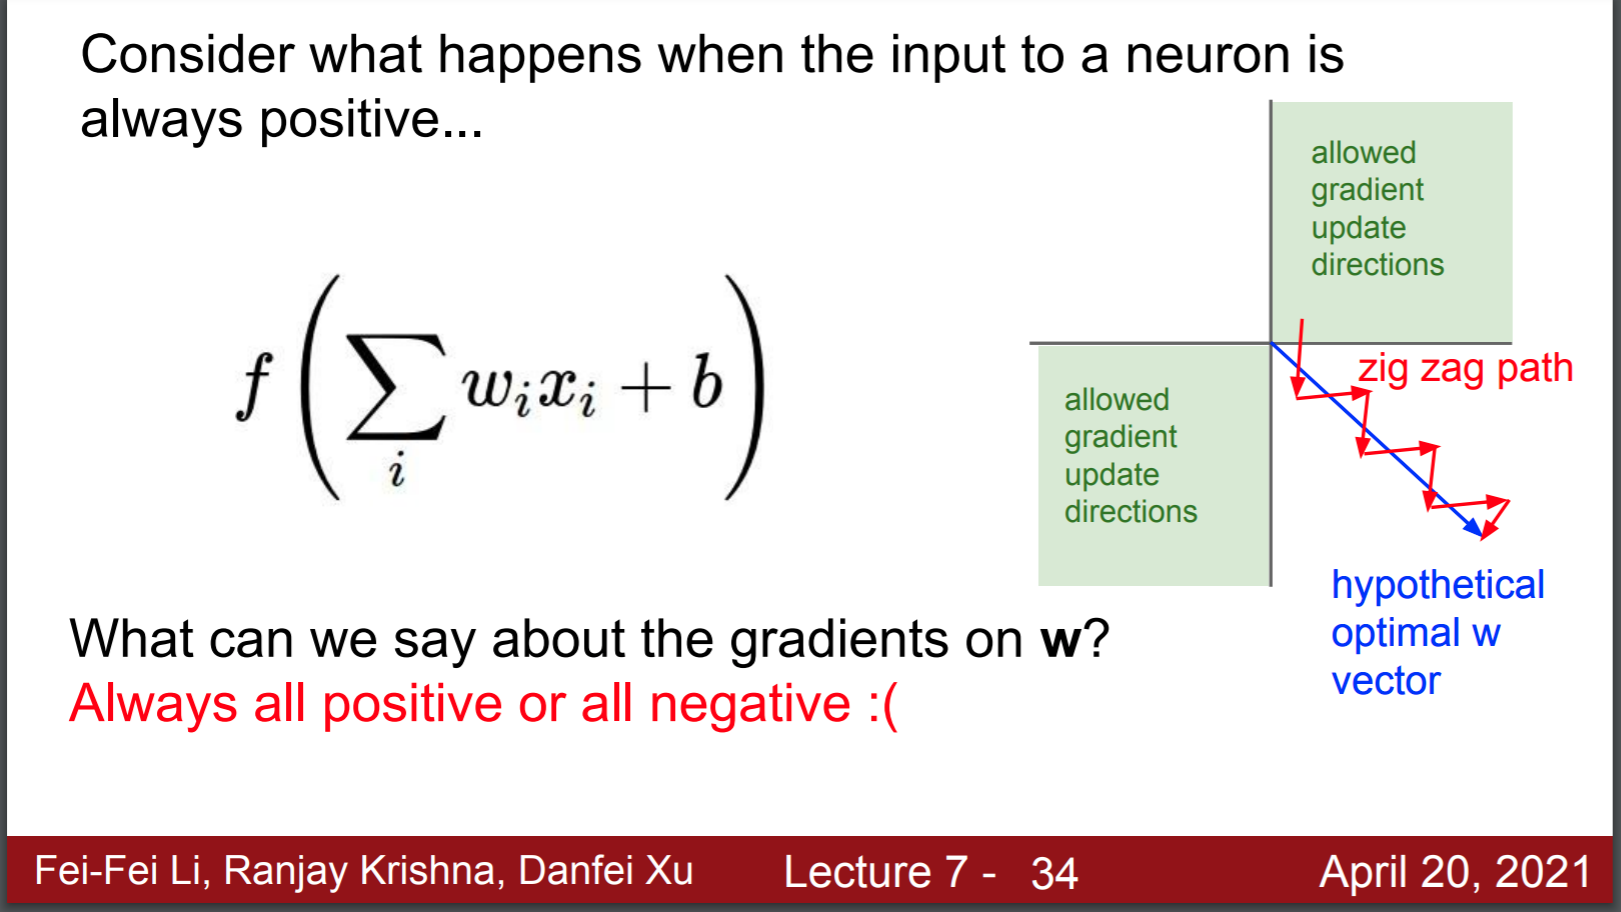
\includegraphics[width=.9\textwidth]{../figure/4-1.png}
    \caption{X始终同号情况下的梯度更新情况}
    \label{img4-1}
\end{figure}

\end{document}